The MiniMax algorithm is a decision rule algorithm for minimizing the
possible loss for a worst case (maximum loss) scenario in a zero sum
game for 2 (or more) players that play in
turns~\cite{Edwards54}.

The algorithm builds a game tree, where each tree node represents a
game state and the children represent the possible game moves that can
be made by either player 1 or player 2.  An evaluation function is
used to compute the score of the board for each leaf of the tree. A
node is a leaf when the game state can no longer be expanded. Finally,
the algorithm recursively minimizes or maximizes the scores of each
node.  To select the best move for player 1, the algorithm picks the
move maximized at the root node.

In CLM, the program starts with a root node (with the initial game state)
that is expanded with the available moves at each level. The graph of the
program is dynamic since nodes are created and then deleted once they are no
longer needed. The latter happens when the
leaf scores are computed or when a node fully minimizes or maximizes the
children scores. When the program ends, only the root node has facts in its
database.

The code in Fig.~\ref{minimax:check-end} deals with the tree expansion process.
The first three rules (lines 1-10) deal
with the case where no children nodes are created and the last three rules
(12-29) deal with the cases for that create new nodes. In particular, the two
rules in lines 12-25 generate new nodes using the
\mytt{exists} language construct, which creates a child node 
\mytt{B}. We link \mytt{B} with its parent (\mytt{parent(B, A)})
and kick start the expansion of that node \mytt{B} by adding a \mytt{play}
fact.

As noted in \sectref{sec:fifo}, the default scheduler is
breadth-first, which in this case leads to a complete expansion of the
tree before computing the scores at the leaves.  This results in using
$\mathcal{O}(n)$ memory, where $n$ is the number of nodes in the tree.

\begin{topfig}
\scriptsize\begin{Verbatim}[numbers=left,commandchars=\\\{\}]
expand(A, Board, [], 0, P, \underline{Depth})
  -o leaf(A, Board).

expand(A, Board, [], N, P, \underline{Depth}),
N > 0, P = player1
  -o maximize(A, N, -00, 0).

expand(A, Board, [], N, P, \underline{Depth}),
N > 0, P = player2
  -o minimize(A, N, +00, 0).

expand(A, Board, [0 | Xs], N, P, Depth),
Depth >= 5
  -o exists B. (\underline{set-static(B)},
       \underline{set-default-priority(B, float(Depth + 1))},
       play(B, Board ++ [P | Xs], next(P), \underline{Depth + 1}),
       expand(A, Board ++ [0], Xs, N + 1, P, \underline{Depth}),
       parent(B, A)).

expand(A, Board, [0 | Xs], N, P, Depth),
Depth < 5
  -o exists B. (\underline{set-default-priority(B, float(Depth + 1))},
       play(B, Board ++ [P | Xs], next(P), \underline{Depth + 1}),
       expand(A, Board ++ [0], Xs, N + 1, P, \underline{Depth}),
       parent(B, A)).

expand(A, Board, [C | Xs], N, P, \underline{Depth})
C <> 0
  -o expand(A, Board ++ [C], Xs, N, P, \underline{Depth}).
\end{Verbatim}
\scap{minimax:check-end}{MiniMax: checking if the game has ended and expanding the tree}
\vspace*{-2ex}
\end{topfig}
\normalsize

With coordination, we set the priority of a node to be its depth (lines 15 and
22) so the tree is expanded in a depth-first fashion,
leading to a memory complexity of $\mathcal{O}(d t)$, where $d$
is the depth of the tree and $t$ is the number of threads.
Since threads prioritize deeper nodes, the scores of the first leaves are immediately
computed and then sent to the parent node. At this point, the leaves are deleted
and reused for other nodes in the tree, resulting in minimal memory usage.

\iffalse
As an example,
consider a system with 2 threads, $T_1$ and $T_2$, where $T_1$ first expands the root
node and then the first child. Since $T_2$ is idle, it steals half of the root's
children nodes and starts expanding one of the nodes in a depth-first fashion.
\fi

\iffalse
\begin{topfig}
   \begin{center}
      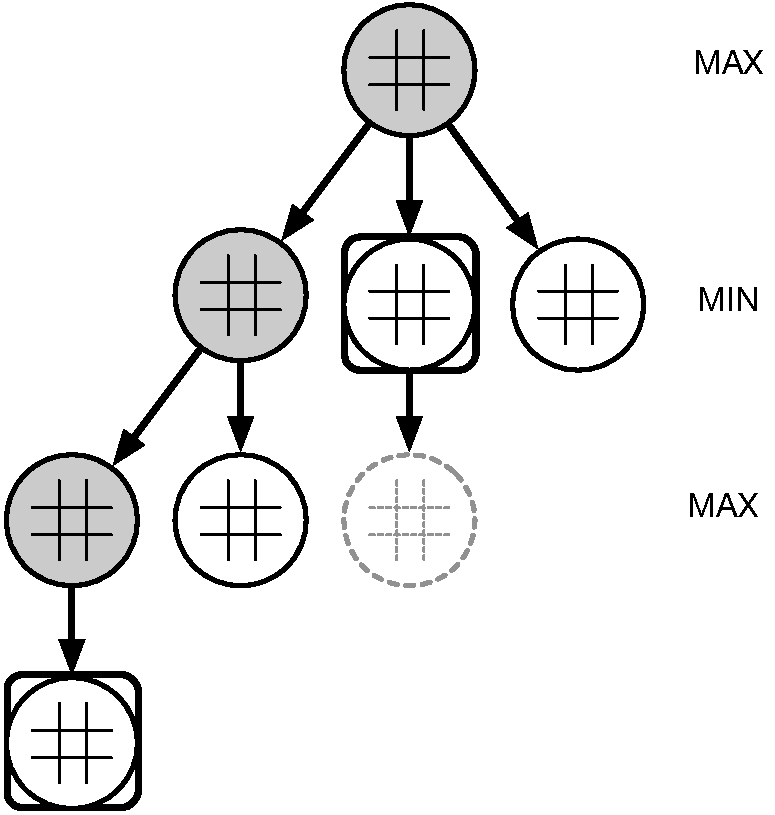
\includegraphics[width=4.5cm]{figures/minimax_tree}
   \end{center}
   \scap{fig:minimax}{Expanding the MiniMax tree using coordination. By prioritizing
      deeper nodes, threads are forced to expand the tree using a depth-first
      approach, which is superior since there is no need to expand the whole
      tree before computing the node scores.}
\end{topfig}
\fi

We also take advantage of memory locality by using \mytt{set-static} (line
14), so that nodes after a certain level are not stolen by other threads. While
this is not critical for performance in shared memory systems where node
stealing is fairly efficient, we expect that such coordination to be critical in
distributed systems.

\begin{topfig}
\vspace*{-3ex}
   \begin{center}
      \subfloat[]{\small\begin{tabular}[b]{ | c | c | c |}
         \hline                       
         \textbf{\# T} & \textbf{R} & \textbf{C} \\ \hline \hline
         1 & 11.80GB & 0.50MB \\ \hline
         2 & 12.19GB & 1.45MB \\ \hline
         4 & 13.82GB & 2.35MB \\ \hline
         8 & 14.87GB & 4.36MB \\ \hline
         16 & 13.79GB & 8.1MB \\ \hline
         \end{tabular}
         \normalsize
      }
      \subfloat[]{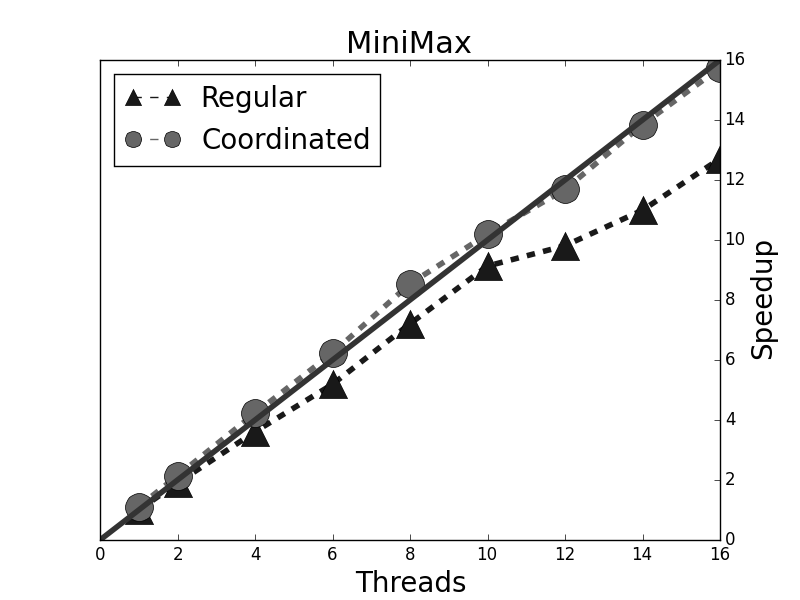
\includegraphics[width=4.5cm]{results/min-max-tictactoe.png}}
   \end{center}
   \scap{results:memory_minmax}{Memory usage and scalability of the regular and coordinated versions
      of MiniMax.}
\vspace*{-2ex}
\end{topfig}

In Fig.~\ref{results:memory_minmax} we compare the memory usage and scalability
of the coordinated MiniMax against the regular MiniMax. The coordinated version
uses significantly less memory (at most 8MB for 16 threads) than the regular
version (almost 14GB). Note that as the number of threads goes
up, memory usage also goes up. This is an artifact of our parallel memory
allocator that allocates large chunks of memory beforehand.
In terms of scalability, our experimental results show a 14-fold speedup for the
coordinated version against a 12-fold for the regular version when using 16
threads. When comparing the two versions directly, there is a 20\% run time
reduction when using 16 threads in the coordinated version.
